% Created by tikzDevice version 0.10.1 on 2017-06-16 09:59:13
% !TEX encoding = UTF-8 Unicode
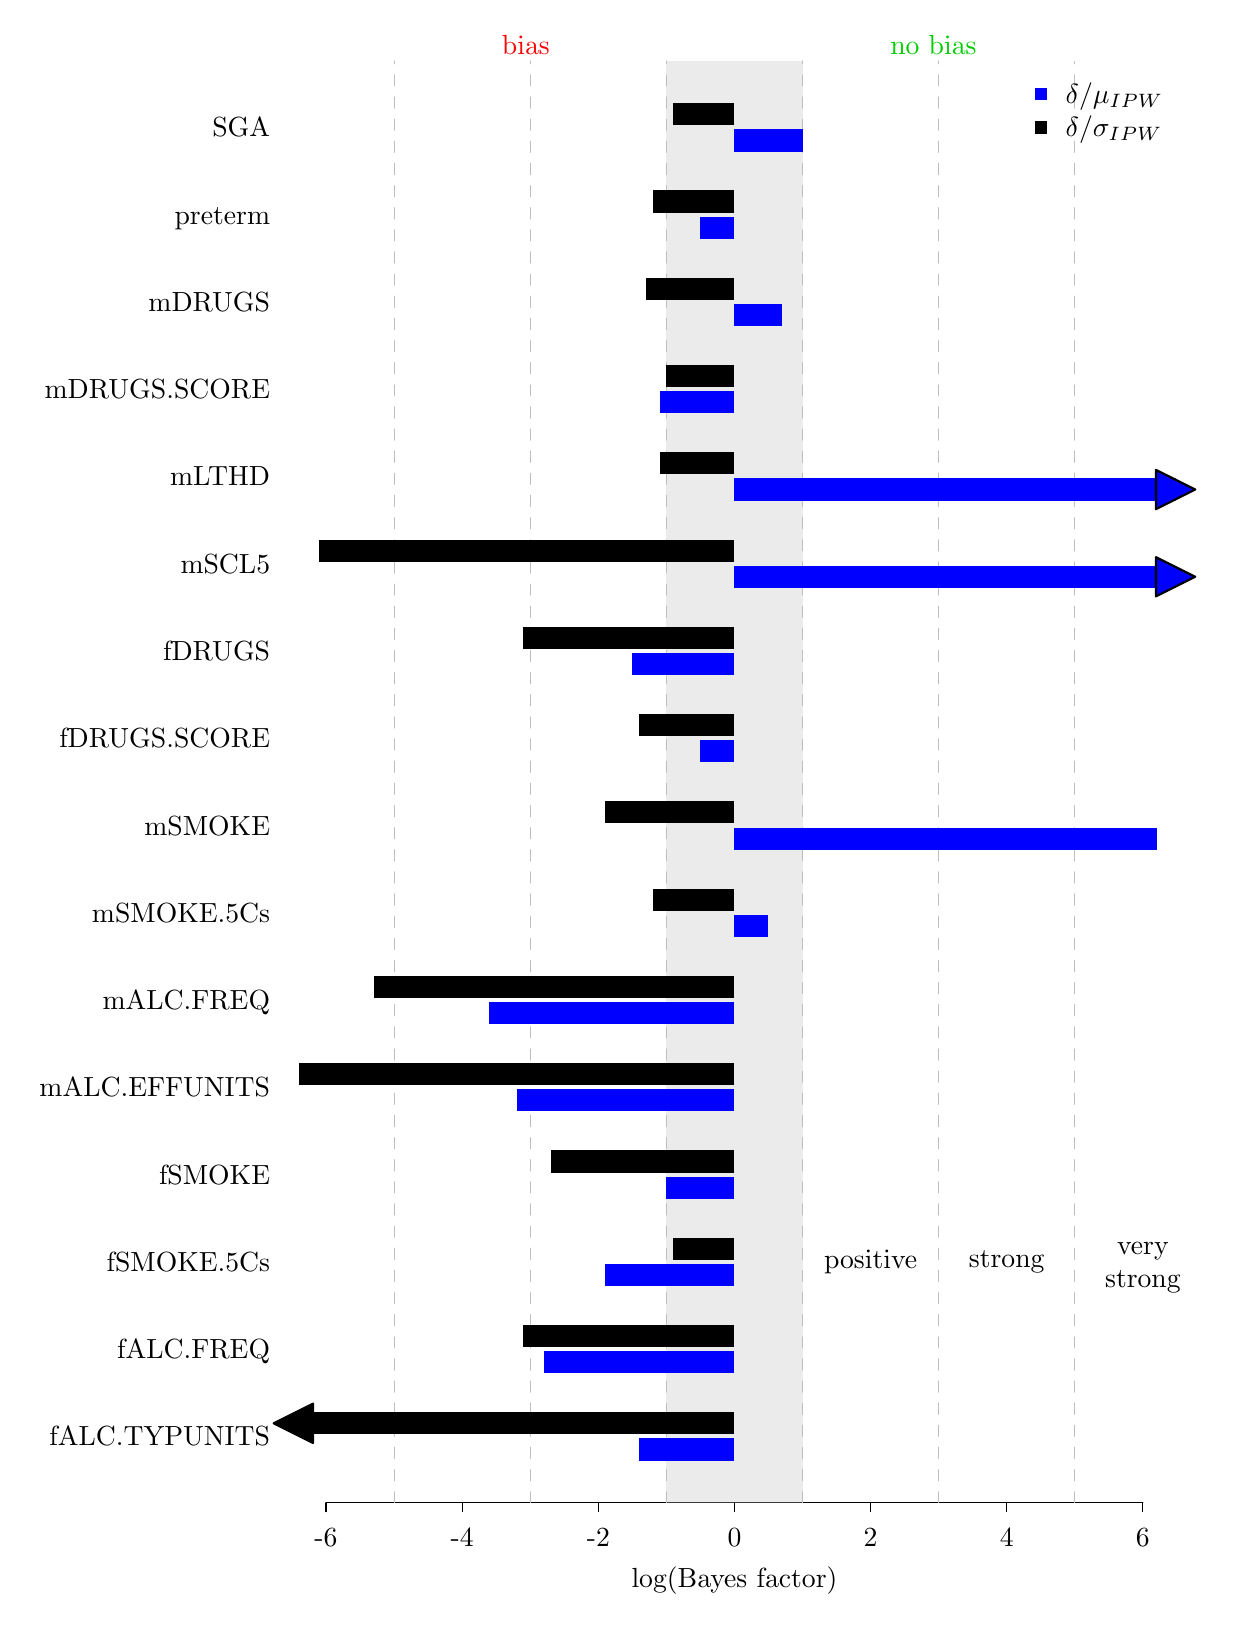
\begin{tikzpicture}[x=1pt,y=1pt]
\definecolor{fillColor}{RGB}{255,255,255}
\path[use as bounding box,fill=fillColor,fill opacity=0.00] (0,0) rectangle (426.79,569.06);
\begin{scope}
\path[clip] (  0.00,  0.00) rectangle (426.79,569.06);
\definecolor{drawColor}{RGB}{0,0,0}

\path[draw=drawColor,line width= 0.4pt,line join=round,line cap=round] (107.81, 36.00) -- (402.98, 36.00);

\path[draw=drawColor,line width= 0.4pt,line join=round,line cap=round] (107.81, 36.00) -- (107.81, 32.81);

\path[draw=drawColor,line width= 0.4pt,line join=round,line cap=round] (157.00, 36.00) -- (157.00, 32.81);

\path[draw=drawColor,line width= 0.4pt,line join=round,line cap=round] (206.20, 36.00) -- (206.20, 32.81);

\path[draw=drawColor,line width= 0.4pt,line join=round,line cap=round] (255.40, 36.00) -- (255.40, 32.81);

\path[draw=drawColor,line width= 0.4pt,line join=round,line cap=round] (304.59, 36.00) -- (304.59, 32.81);

\path[draw=drawColor,line width= 0.4pt,line join=round,line cap=round] (353.79, 36.00) -- (353.79, 32.81);

\path[draw=drawColor,line width= 0.4pt,line join=round,line cap=round] (402.98, 36.00) -- (402.98, 32.81);

\node[text=drawColor,anchor=base,inner sep=0pt, outer sep=0pt, scale=  1.00] at (107.81, 20.40) {-6};

\node[text=drawColor,anchor=base,inner sep=0pt, outer sep=0pt, scale=  1.00] at (157.00, 20.40) {-4};

\node[text=drawColor,anchor=base,inner sep=0pt, outer sep=0pt, scale=  1.00] at (206.20, 20.40) {-2};

\node[text=drawColor,anchor=base,inner sep=0pt, outer sep=0pt, scale=  1.00] at (255.40, 20.40) {0};

\node[text=drawColor,anchor=base,inner sep=0pt, outer sep=0pt, scale=  1.00] at (304.59, 20.40) {2};

\node[text=drawColor,anchor=base,inner sep=0pt, outer sep=0pt, scale=  1.00] at (353.79, 20.40) {4};

\node[text=drawColor,anchor=base,inner sep=0pt, outer sep=0pt, scale=  1.00] at (402.98, 20.40) {6};
\end{scope}
\begin{scope}
\path[clip] (  0.00,  0.00) rectangle (426.79,569.06);
\definecolor{drawColor}{RGB}{0,0,0}

\node[text=drawColor,anchor=base,inner sep=0pt, outer sep=0pt, scale=  1.00] at (255.40,  5.40) {log(Bayes factor)};
\end{scope}
\begin{scope}
\path[clip] ( 96.00, 36.00) rectangle (414.79,557.06);
\definecolor{fillColor}{RGB}{190,190,190}

\path[fill=fillColor,fill opacity=0.30] (230.80, 36.00) rectangle (279.99,557.06);
\definecolor{drawColor}{RGB}{190,190,190}

\path[draw=drawColor,line width= 0.4pt,dash pattern=on 4pt off 4pt ,line join=round,line cap=round] (279.99, 36.00) -- (279.99,557.06);

\path[draw=drawColor,line width= 0.4pt,dash pattern=on 4pt off 4pt ,line join=round,line cap=round] (230.80, 36.00) -- (230.80,557.06);

\path[draw=drawColor,line width= 0.4pt,dash pattern=on 4pt off 4pt ,line join=round,line cap=round] (329.19, 36.00) -- (329.19,557.06);

\path[draw=drawColor,line width= 0.4pt,dash pattern=on 4pt off 4pt ,line join=round,line cap=round] (181.60, 36.00) -- (181.60,557.06);

\path[draw=drawColor,line width= 0.4pt,dash pattern=on 4pt off 4pt ,line join=round,line cap=round] (378.39, 36.00) -- (378.39,557.06);

\path[draw=drawColor,line width= 0.4pt,dash pattern=on 4pt off 4pt ,line join=round,line cap=round] (132.41, 36.00) -- (132.41,557.06);
\end{scope}
\begin{scope}
\path[clip] (  0.00,  0.00) rectangle (426.79,569.06);
\definecolor{drawColor}{RGB}{255,0,0}

\node[text=drawColor,anchor=base,inner sep=0pt, outer sep=0pt, scale=  1.00] at (180.02,559.46) {bias};
\definecolor{drawColor}{RGB}{0,205,0}

\node[text=drawColor,anchor=base east,inner sep=0pt, outer sep=0pt, scale=  1.00] at (342.88,559.46) {no bias};
\definecolor{drawColor}{RGB}{0,0,0}

\node[text=drawColor,anchor=base east,inner sep=0pt, outer sep=0pt, scale=  1.00] at ( 87.60, 56.58) {fALC.TYPUNITS};

\node[text=drawColor,anchor=base east,inner sep=0pt, outer sep=0pt, scale=  1.00] at ( 87.60, 88.12) {fALC.FREQ};

\node[text=drawColor,anchor=base east,inner sep=0pt, outer sep=0pt, scale=  1.00] at ( 87.60,119.65) {fSMOKE.5Cs};

\node[text=drawColor,anchor=base east,inner sep=0pt, outer sep=0pt, scale=  1.00] at ( 87.60,151.18) {fSMOKE};

\node[text=drawColor,anchor=base east,inner sep=0pt, outer sep=0pt, scale=  1.00] at ( 87.60,182.72) {mALC.EFFUNITS};

\node[text=drawColor,anchor=base east,inner sep=0pt, outer sep=0pt, scale=  1.00] at ( 87.60,214.25) {mALC.FREQ};

\node[text=drawColor,anchor=base east,inner sep=0pt, outer sep=0pt, scale=  1.00] at ( 87.60,245.78) {mSMOKE.5Cs};

\node[text=drawColor,anchor=base east,inner sep=0pt, outer sep=0pt, scale=  1.00] at ( 87.60,277.32) {mSMOKE};

\node[text=drawColor,anchor=base east,inner sep=0pt, outer sep=0pt, scale=  1.00] at ( 87.60,308.85) {fDRUGS.SCORE};

\node[text=drawColor,anchor=base east,inner sep=0pt, outer sep=0pt, scale=  1.00] at ( 87.60,340.38) {fDRUGS};

\node[text=drawColor,anchor=base east,inner sep=0pt, outer sep=0pt, scale=  1.00] at ( 87.60,371.92) {mSCL5};

\node[text=drawColor,anchor=base east,inner sep=0pt, outer sep=0pt, scale=  1.00] at ( 87.60,403.45) {mLTHD};

\node[text=drawColor,anchor=base east,inner sep=0pt, outer sep=0pt, scale=  1.00] at ( 87.60,434.98) {mDRUGS.SCORE};

\node[text=drawColor,anchor=base east,inner sep=0pt, outer sep=0pt, scale=  1.00] at ( 87.60,466.52) {mDRUGS};

\node[text=drawColor,anchor=base east,inner sep=0pt, outer sep=0pt, scale=  1.00] at ( 87.60,498.05) {preterm};

\node[text=drawColor,anchor=base east,inner sep=0pt, outer sep=0pt, scale=  1.00] at ( 87.60,529.58) {SGA};
\end{scope}
\begin{scope}
\path[clip] ( 96.00, 36.00) rectangle (414.79,557.06);
\definecolor{drawColor}{RGB}{0,0,255}

\path[draw=drawColor,line width= 8.0pt,line join=round] (255.40,528.30) -- (279.99,528.30);

\path[draw=drawColor,line width= 8.0pt,line join=round] (255.40,496.76) -- (243.10,496.76);

\path[draw=drawColor,line width= 8.0pt,line join=round] (255.40,465.23) -- (272.61,465.23);

\path[draw=drawColor,line width= 8.0pt,line join=round] (255.40,433.70) -- (228.34,433.70);

\path[draw=drawColor,line width= 8.0pt,line join=round] (255.40,402.16) -- (426.79,402.16);

\path[draw=drawColor,line width= 8.0pt,line join=round] (255.40,370.63) -- (426.79,370.63);

\path[draw=drawColor,line width= 8.0pt,line join=round] (255.40,339.10) -- (218.50,339.10);

\path[draw=drawColor,line width= 8.0pt,line join=round] (255.40,307.56) -- (243.10,307.56);

\path[draw=drawColor,line width= 8.0pt,line join=round] (255.40,276.03) -- (407.90,276.03);

\path[draw=drawColor,line width= 8.0pt,line join=round] (255.40,244.50) -- (267.69,244.50);

\path[draw=drawColor,line width= 8.0pt,line join=round] (255.40,212.96) -- (166.84,212.96);

\path[draw=drawColor,line width= 8.0pt,line join=round] (255.40,181.43) -- (176.68,181.43);

\path[draw=drawColor,line width= 8.0pt,line join=round] (255.40,149.90) -- (230.80,149.90);

\path[draw=drawColor,line width= 8.0pt,line join=round] (255.40,118.36) -- (208.66,118.36);

\path[draw=drawColor,line width= 8.0pt,line join=round] (255.40, 86.83) -- (186.52, 86.83);

\path[draw=drawColor,line width= 8.0pt,line join=round] (255.40, 55.30) -- (220.96, 55.30);
\definecolor{drawColor}{RGB}{0,0,0}

\path[draw=drawColor,line width= 8.0pt,line join=round] (255.40,537.76) -- (233.26,537.76);

\path[draw=drawColor,line width= 8.0pt,line join=round] (255.40,506.22) -- (225.88,506.22);

\path[draw=drawColor,line width= 8.0pt,line join=round] (255.40,474.69) -- (223.42,474.69);

\path[draw=drawColor,line width= 8.0pt,line join=round] (255.40,443.16) -- (230.80,443.16);

\path[draw=drawColor,line width= 8.0pt,line join=round] (255.40,411.62) -- (228.34,411.62);

\path[draw=drawColor,line width= 8.0pt,line join=round] (255.40,380.09) -- (105.35,380.09);

\path[draw=drawColor,line width= 8.0pt,line join=round] (255.40,348.56) -- (179.14,348.56);

\path[draw=drawColor,line width= 8.0pt,line join=round] (255.40,317.02) -- (220.96,317.02);

\path[draw=drawColor,line width= 8.0pt,line join=round] (255.40,285.49) -- (208.66,285.49);

\path[draw=drawColor,line width= 8.0pt,line join=round] (255.40,253.96) -- (225.88,253.96);

\path[draw=drawColor,line width= 8.0pt,line join=round] (255.40,222.42) -- (125.03,222.42);

\path[draw=drawColor,line width= 8.0pt,line join=round] (255.40,190.89) -- ( 97.97,190.89);

\path[draw=drawColor,line width= 8.0pt,line join=round] (255.40,159.36) -- (188.98,159.36);

\path[draw=drawColor,line width= 8.0pt,line join=round] (255.40,127.82) -- (233.26,127.82);

\path[draw=drawColor,line width= 8.0pt,line join=round] (255.40, 96.29) -- (179.14, 96.29);

\path[draw=drawColor,line width= 8.0pt,line join=round] (255.40, 64.76) -- ( 93.05, 64.76);
\end{scope}
\begin{scope}
\path[clip] (  0.00,  0.00) rectangle (426.79,569.06);
\definecolor{drawColor}{RGB}{0,0,0}

\node[text=drawColor,anchor=base,inner sep=0pt, outer sep=0pt, scale=  1.00] at (304.59,120.75) {positive};

\node[text=drawColor,anchor=base,inner sep=0pt, outer sep=0pt, scale=  1.00] at (353.79,120.99) {strong};

\node[text=drawColor,anchor=base,inner sep=0pt, outer sep=0pt, scale=  1.00] at (402.98,125.65) {very};

\node[text=drawColor,anchor=base,inner sep=0pt, outer sep=0pt, scale=  1.00] at (402.98,113.65) { strong};
\definecolor{fillColor}{RGB}{0,0,255}

\path[draw=drawColor,line width= 0.8pt,line join=round,line cap=round,fill=fillColor] (407.71,395.08) --
	(421.87,402.16) --
	(407.71,409.24) --
	cycle;

\path[draw=drawColor,line width= 0.8pt,line join=round,line cap=round,fill=fillColor] (407.71,363.55) --
	(421.87,370.63) --
	(407.71,377.71) --
	cycle;
\definecolor{fillColor}{RGB}{0,0,0}

\path[draw=drawColor,line width= 0.8pt,line join=round,line cap=round,fill=fillColor] (103.08, 71.84) --
	( 88.92, 64.76) --
	(103.08, 57.68) --
	cycle;
\definecolor{drawColor}{RGB}{255,255,255}

\path[draw=drawColor,line width= 0.4pt,line join=round,line cap=round] (357.09,557.06) rectangle (414.79,521.06);
\definecolor{fillColor}{RGB}{0,0,255}

\path[fill=fillColor] (363.84,542.81) --
	(368.34,542.81) --
	(368.34,547.31) --
	(363.84,547.31) --
	cycle;
\definecolor{fillColor}{RGB}{0,0,0}

\path[fill=fillColor] (363.84,530.81) --
	(368.34,530.81) --
	(368.34,535.31) --
	(363.84,535.31) --
	cycle;
\definecolor{drawColor}{RGB}{0,0,0}

\node[text=drawColor,anchor=base west,inner sep=0pt, outer sep=0pt, scale=  1.00] at (375.09,541.61) {$\delta/\mu_{IPW}$};

\node[text=drawColor,anchor=base west,inner sep=0pt, outer sep=0pt, scale=  1.00] at (375.09,529.61) {$\delta/\sigma_{IPW}$};
\end{scope}
\end{tikzpicture}
